% !TeX program = xelatex
% AI for Theological Inquiry — Lecture 3 deck. Build: xelatex lecture03.tex (twice).
% beamer-slides house preamble.
% Copy into a new deck and edit \deckauthor / \deckemail / \deckdate / colors.
% Build: xelatex deck.tex (run twice). See ../SKILL.md for the full house style.
\documentclass[aspectratio=169,11pt]{beamer}

\usetheme{metropolis}
\usepackage{fontspec}
\usepackage{graphicx}
\usepackage{tikz}
\usetikzlibrary{arrows.meta,positioning,shapes.geometric,fit,shadows}
\usepackage{tcolorbox}
\tcbuselibrary{skins,breakable}
\usepackage{fontawesome5}
\usepackage{listings}
\usepackage{booktabs}
\usepackage{array}

% ---------------------------------------------------------------- palette
% Placeholder professional navy/accent palette — swap for the exact ANL/ALCF
% brand hex values if you have the brand guide; do not present these as
% "official" institutional colors.
\definecolor{labnavy}{RGB}{18,42,73}
\definecolor{labink}{RGB}{40,44,52}
\definecolor{accentgold}{RGB}{223,161,54}
\definecolor{accentteal}{RGB}{0,137,123}
\definecolor{accentblue}{RGB}{41,98,168}
\definecolor{lightgray}{RGB}{245,246,248}
\definecolor{midgray}{RGB}{110,118,129}

% Hard rule: background is always white.
\setbeamercolor{background canvas}{bg=white}
\setbeamercolor{palette primary}{bg=labnavy,fg=white}
\setbeamercolor{frametitle}{bg=labnavy,fg=white}
\setbeamercolor{progress bar}{fg=accentteal,bg=lightgray}
\setbeamercolor{normal text}{fg=labink}
\setbeamercolor{alerted text}{fg=accentgold}
\setbeamercolor{footline}{fg=midgray}
\setbeamerfont{footline}{size=\tiny}

% Tighter default itemize indentation (see SKILL.md Gotchas — do NOT pass
% [leftmargin=...] to Beamer's itemize, that slot is for overlay specs).
\setlength{\leftmargini}{14pt}

% ---------------------------------------------------------------- deck metadata
% Fill these in per-deck. Email + date are a hard rule on the title page.
\newcommand{\deckauthor}{Huihuo Zheng}
\newcommand{\deckemail}{huihuo.zheng@wheaton.edu}
\newcommand{\deckinstitute}{Wheaton College}
% \date{...} still needs to be called explicitly in the document, e.g. \date{\today}

% ---------------------------------------------------------------- logo
% Looks for a real logo file first; falls back to a plain text lockup rather
% than fabricating the institutional mark. Put the real file at
% logos/argonne_logo.pdf (or .png) next to the deck, or point this at a
% shared assets/logos/ path.
% Drop a real logo at logos/wheaton_logo.pdf (or .png) to use it; otherwise
% this falls back to a plain text lockup rather than fabricating the mark.
\newcommand{\decklogo}[1][0.16\textwidth]{%
  \IfFileExists{logos/wheaton_logo.pdf}%
    {
\includegraphics[width=#1]{logos/wheaton_logo.pdf}}%
    {\IfFileExists{logos/wheaton_logo.png}%
      {
\includegraphics[width=#1]{logos/wheaton_logo.png}}%
      {\begin{minipage}{#1}\centering
         {\Large\bfseries\textsc{\textcolor{labnavy}{Wheaton}}}\\[1pt]
         {\small\bfseries\textsc{\textcolor{labnavy}{College}}}
       \end{minipage}}}%
}

% Small corner logo on every content slide (title page uses \decklogo directly
% instead, usually larger — see templates/titlepage.tex). Comment out this
% \logo{} line if you don't want the small footer/corner logo repeated.
% Teaching deck: no repeated corner logo (title page carries it once).
% \logo{\IfFileExists{logos/argonne_logo.pdf}%
%   {\includegraphics[height=0.45cm]{logos/argonne_logo.pdf}}%
%   {\IfFileExists{logos/argonne_logo.png}%
%     {\includegraphics[height=0.45cm]{logos/argonne_logo.png}}{}}}

% ---------------------------------------------------------------- shadowed boxes
% House rule: every box gets a shadow. Pick "drop shadow" (crisp) or
% "drop fuzzy shadow" (soft) and use it consistently through one deck.
% IMPORTANT: "enhanced" is required for the shadow to render at all — without
% it tcolorbox silently accepts the "drop shadow"/"drop fuzzy shadow" key and
% draws nothing (no error, no warning). See SKILL.md Gotchas.
\newtcolorbox{featbox}[2]{
  enhanced,
  colback=lightgray, colframe=#1, boxrule=0.6pt, arc=3pt,
  left=6pt, right=6pt, top=4pt, bottom=4pt,
  title=#2, colbacktitle=#1, coltitle=white,
  fonttitle=\bfseries\small, boxsep=1pt,
  drop fuzzy shadow
}

\newtcolorbox{calloutbox}[1][labnavy]{
  enhanced,
  colback=#1!6, colframe=#1, boxrule=0.6pt, arc=3pt,
  left=10pt, right=10pt, top=6pt, bottom=6pt,
  drop fuzzy shadow
}

\lstdefinestyle{shell}{
  basicstyle=\ttfamily\scriptsize\color{labink},
  keywordstyle=\color{accentblue}\bfseries,
  commentstyle=\color{midgray}\itshape,
  stringstyle=\color{accentteal},
  backgroundcolor=\color{lightgray},
  frame=single, framerule=0.4pt, rulecolor=\color{midgray!60},
  breaklines=true, columns=fullflexible,
  xleftmargin=4pt, xrightmargin=4pt, framexleftmargin=4pt
}


% ---- palette aliases for this deck's three pillars (match lecture01/02) ----
\definecolor{cAgent}{RGB}{41,98,168}   % agentic AI  (blue)
\definecolor{cRAG}{RGB}{0,137,123}     % RAG         (teal)
\definecolor{cEval}{RGB}{223,161,54}   % evaluation  (gold)

\title{AI for Theological Inquiry}
\subtitle{Lecture 3 — Coding agents on an open model, \& vibe coding}
\date{September 15, 2026}

\begin{document}

% beamer-slides house title page.
% Requires preamble.tex to be loaded first (\decklogo, \deckauthor, \deckemail,
% \deckinstitute). Set \title{}/\subtitle{} and \date{} before this frame.
%
% Hard rule: title page always shows author name, email, and date. Email sits
% bottom-left in small type, footnote-style — not in the author block.

\begin{frame}[plain]
  \begin{columns}[c]
    \begin{column}{0.32\textwidth}
      \centering
      \decklogo[0.9\textwidth]
    \end{column}
    \begin{column}{0.66\textwidth}
      {\usebeamerfont{title}\usebeamercolor[fg]{title}\Huge\bfseries \inserttitle\par}
      \ifx\insertsubtitle\@empty\else
        \vspace{4pt}
        {\large\color{midgray}\insertsubtitle\par}
      \fi
      \vspace{18pt}
      {\small
        \deckauthor\\
        \deckinstitute\\
        \insertdate}
    \end{column}
  \end{columns}
  \vfill
  {\footnotesize\color{midgray}\deckemail\par}
\end{frame}


% ---------------------------------------------------------------- recap / where we are
\begin{frame}{Where we are: put the agent loop back around the box}
  \begin{columns}[c, totalwidth=\textwidth]
    \begin{column}{0.47\textwidth}
      \begin{featbox}{accentblue}{\faCheckCircle\ Last week}
        \small
        \begin{itemize}
          \item Opened the hood on the \textbf{raw model}
          \item One call in, one answer out
          \item \textbf{Caught it inventing a verse}
        \end{itemize}
        {\scriptsize\color{midgray}You met the engine --- and its limits.}
      \end{featbox}
    \end{column}
    \begin{column}{0.06\textwidth}\end{column}
    \begin{column}{0.47\textwidth}
      \begin{featbox}{cAgent}{\faRobot\ This week}
        \small
        \begin{itemize}
          \item Wrap the \textbf{plan $\to$ act $\to$ observe} loop back on
          \item Drive it from a \textbf{coding agent} (opencode)
          \item \dots\ on the \textbf{same open ALCF model}
        \end{itemize}
        {\scriptsize\color{midgray}The engine, now in a car that drives itself.}
      \end{featbox}
    \end{column}
  \end{columns}
  \vspace{10pt}
  \begin{center}\small\color{labnavy}\bfseries
    Week 2 = the engine. This week = the engine \emph{plus a loop} --- and learning to steer.\end{center}
\end{frame}

% ---------------------------------------------------------------- agenda
\begin{frame}{Today: wire up a coding agent, then learn to distrust it}
  \begin{columns}[t, totalwidth=\textwidth]
    \begin{column}{0.47\textwidth}
      \begin{featbox}{accentblue}{\faLaptopCode\ Part 1 --- Connect}
        \small
        \begin{itemize}
          \item What a \textbf{coding agent} is (the loop, again)
          \item ``It's just an OpenAI-compatible URL''
          \item \texttt{opencode.json}: one config block
          \item Launch $\to$ pick the ALCF model $\to$ run
        \end{itemize}
      \end{featbox}
    \end{column}
    \begin{column}{0.06\textwidth}\end{column}
    \begin{column}{0.47\textwidth}
      \begin{featbox}{accentgold}{\faMagic\ Part 2 --- Vibe coding}
        \small
        \begin{itemize}
          \item What ``vibe coding'' is --- and why it's fast
          \item Build a small tool by \emph{describing} it
          \item Trip the factual trap on purpose
          \item Vibe to explore, \textbf{verify} to publish
        \end{itemize}
      \end{featbox}
    \end{column}
  \end{columns}
  \vspace{8pt}
  \begin{center}\small\color{midgray}%
    $\sim$20 min concept $\cdot$ $\sim$25 min connect-lab $\cdot$ $\sim$30 min vibe-lab $\cdot$ $\sim$15 min discipline.\end{center}
\end{frame}

% ---------------------------------------------------------------- what is a coding agent
\begin{frame}{A coding agent is the loop, doing real work}
  \begin{center}
  \begin{tikzpicture}[font=\scriptsize,
      node distance=0.7cm,
      stg/.style={rectangle, rounded corners=3pt, draw, thick, fill=lightgray,
                  drop shadow, align=center, text width=1.55cm, minimum height=0.7cm}]
    \node[stg, draw=labnavy]  (goal)    {\faBullseye\\ Goal};
    \node[stg, draw=cAgent, right=of goal] (plan) {\faSitemap\\ Plan};
    \node[stg, draw=cRAG, right=of plan]   (act)  {\faTools\\ Act\\ \scriptsize(edit/run)};
    \node[stg, draw=accentblue, right=of act] (obs) {\faEye\\ Observe\\ \scriptsize(result)};
    \node[stg, draw=cEval, right=of obs] (ans) {\faCheckDouble\\ Done};
    \draw[-{Latex[length=6pt]}, thick, midgray] (goal) -- (plan);
    \draw[-{Latex[length=6pt]}, thick, midgray] (plan) -- (act);
    \draw[-{Latex[length=6pt]}, thick, midgray] (act)  -- (obs);
    \draw[-{Latex[length=6pt]}, thick, midgray] (obs) -- (ans);
    \draw[-{Latex[length=6pt]}, thick, cAgent] (obs.south) to[out=-90,in=-90]
      node[below,font=\scriptsize]{not done? loop back} (plan.south);
  \end{tikzpicture}
  \end{center}
  \vspace{6pt}
  \begin{columns}[t, totalwidth=\textwidth]
    \begin{column}{0.48\textwidth}
      \begin{featbox}{accentblue}{\faTerminal\ What opencode is}
        \scriptsize A \textbf{free, open-source} coding agent in your terminal.
        It reads \& writes files and runs commands --- looping until the goal is met.
        Same family as Claude Code (Wk 1), but \textbf{open} and \textbf{provider-agnostic}.
      \end{featbox}
    \end{column}
    \begin{column}{0.04\textwidth}\end{column}
    \begin{column}{0.48\textwidth}
      \begin{featbox}{cRAG}{\faKey\ Why it matters here}
        \scriptsize We point it at the \textbf{same open model on ALCF} from Week 2 ---
        no vendor key, nothing leaves for a company. The stack stays \textbf{disclosable}.
      \end{featbox}
    \end{column}
  \end{columns}
\end{frame}

% ---------------------------------------------------------------- the connect trick
\begin{frame}{The whole trick: the ALCF endpoint is ``just a URL''}
  \begin{center}
  \begin{tikzpicture}[font=\scriptsize,
      s/.style={rectangle, rounded corners=3pt, draw, thick, fill=lightgray,
                drop shadow, align=center, text width=2.6cm, minimum height=1.15cm}]
    \node[s, draw=accentblue] (oc)  {\faTerminal\\ \textbf{opencode}\\ \scriptsize the agent (loop)};
    \node[s, draw=cRAG, right=1.3cm of oc] (url) {\faLink\\ \textbf{OpenAI-compatible}\\ \scriptsize \texttt{/v1/chat/...}};
    \node[s, draw=cAgent, right=1.3cm of url] (alcf) {\faServer\\ \textbf{ALCF endpoint}\\ \scriptsize open-weight model};
    \draw[-{Latex[length=5pt]}, thick, midgray] (oc)--(url) node[midway,above,font=\scriptsize,text=midgray]{same URL};
    \draw[-{Latex[length=5pt]}, thick, midgray] (url)--(alcf) node[midway,above,font=\scriptsize,text=midgray]{your token};
  \end{tikzpicture}
  \end{center}
  \vspace{6pt}
  \begin{columns}[t, totalwidth=\textwidth]
    \begin{column}{0.48\textwidth}
      \begin{featbox}{cAgent}{\faCheckCircle\ You already know the hard part}
        \scriptsize The \texttt{base\_url} and the token are \textbf{the same} as your
        Week 2 client. A coding agent is just a nicer front-end over that call.
      \end{featbox}
    \end{column}
    \begin{column}{0.04\textwidth}\end{column}
    \begin{column}{0.48\textwidth}
      \begin{featbox}{accentblue}{\faPuzzlePiece\ Three fields to set}
        \scriptsize \texttt{baseURL} (unchanged) $\cdot$ \texttt{apiKey} (your ALCF
        token, via an env var) $\cdot$ a real \texttt{model} ID from
        \texttt{list-endpoints}.
      \end{featbox}
    \end{column}
  \end{columns}
  \vspace{6pt}
  \begin{center}\small\color{labnavy}\bfseries
    opencode talks to \emph{any} OpenAI-compatible provider --- ALCF is one of them.\end{center}
\end{frame}

% ---------------------------------------------------------------- step 1: token
\begin{frame}[fragile]{Step 1 --- Give opencode a fresh token (each session)}
  \begin{columns}[t, totalwidth=\textwidth]
    \begin{column}{0.52\textwidth}
      {\footnotesize\bfseries\color{accentblue}\faKey\ Export the token into your shell}
      \begin{lstlisting}[style=shell]
# same helper as Week 2 (browser login once)
export ALCF_TOKEN="$(python \
  inference_auth_token.py get_access_token)"

# convenience script does exactly this:
source set_alcf_token.sh
      \end{lstlisting}
    \end{column}
    \begin{column}{0.48\textwidth}
      {\footnotesize\bfseries\color{cRAG}\faList\ Confirm a live model ID}
      \begin{lstlisting}[style=shell]
curl -s https://inference-api.alcf.anl.gov/\
resource_server/list-endpoints \
  -H "Authorization: Bearer $ALCF_TOKEN"
      \end{lstlisting}
      {\scriptsize\color{midgray}Copy an exact ID --- you'll paste it into the config.}
    \end{column}
  \end{columns}
  \vspace{6pt}
  \begin{calloutbox}[accentgold]
    \small\faExclamationTriangle\ opencode reads the token \textbf{once, at startup}.
    When calls start returning \textbf{401}, refresh the env var \emph{and restart}
    opencode. That's not a bug --- the token just expired ($\sim$48\,h).
  \end{calloutbox}
\end{frame}

% ---------------------------------------------------------------- step 2: the config
\begin{frame}[fragile]{Step 2 --- Tell opencode about ALCF (\texttt{opencode.json})}
  \begin{lstlisting}[style=shell, title={opencode.json --- one provider, a menu of models}]
{
  "model": "alcf/meta-llama/Meta-Llama-3.1-8B-Instruct",   // default at startup
  "provider": { "alcf": {
    "npm": "@ai-sdk/openai-compatible",
    "options": {
      "baseURL": "https://inference-api.alcf.anl.gov/resource_server/sophia/vllm/v1",
      "apiKey": "{env:ALCF_TOKEN}"
    },
    "models": {                       // every ID here appears in /models
      "meta-llama/Meta-Llama-3.1-8B-Instruct": {},
      "meta-llama/Llama-3.3-70B-Instruct":     {},
      "openai/gpt-oss-120b":                   {}
    }
  } }
}
  \end{lstlisting}
  \begin{center}\scriptsize\color{midgray}%
    Same \texttt{baseURL} \& token as Week 2 $\cdot$ list as many \textbf{served} chat models as you like --- each becomes a choice.\end{center}
\end{frame}

% ---------------------------------------------------------------- step 3: launch
\begin{frame}[fragile]{Step 3 --- Launch, pick the model, run your first agent}
  \begin{columns}[t, totalwidth=\textwidth]
    \begin{column}{0.5\textwidth}
      {\footnotesize\bfseries\color{accentblue}\faPlay\ Start it}
      \begin{lstlisting}[style=shell]
opencode          # in the project folder

# inside opencode:
/models    # menu of ALL models you listed
           # re-run any time to switch
      \end{lstlisting}
      {\scriptsize\color{midgray}Sanity check: \emph{``What model are you, and who serves you?''}}
    \end{column}
    \begin{column}{0.5\textwidth}
      \begin{featbox}{cRAG}{\faRandom\ Pick --- and switch}
        \scriptsize \texttt{/models} lists every model from your config. Start with
        \textbf{8B} (fast, and usefully \emph{fallible}); switch to \textbf{70B} or
        \texttt{gpt-oss-120b} for harder code. Same agent, same loop --- one keystroke.
      \end{featbox}
    \end{column}
  \end{columns}
  \vspace{6pt}
  \begin{center}\small\color{labnavy}\bfseries
    From here on, you \emph{describe}; the agent plans, writes, runs, and self-corrects.\end{center}
\end{frame}

% ================================================================ PART 2 — vibe coding
\begin{frame}{Part 2 --- ``Vibe coding'': describe it, let the agent build it}
  \vspace{2pt}
  \begin{calloutbox}[accentgold]
    \small\faQuoteLeft\ \textbf{Vibe coding} (Karpathy, 2025): say what you want in
    plain language, let the agent write \& run the code, and \emph{``give in to the
    vibes''} --- accepting output \textbf{without reading every line}.
  \end{calloutbox}
  \vspace{8pt}
  \begin{columns}[t, totalwidth=\textwidth]
    \begin{column}{0.48\textwidth}
      \begin{featbox}{cRAG}{\faBolt\ Why it's seductive --- and real}
        \scriptsize Prototype in \textbf{minutes}. A low barrier: \emph{describe}, don't
        syntax. Genuinely great for \textbf{throwaway exploration} and learning.
      \end{featbox}
    \end{column}
    \begin{column}{0.04\textwidth}\end{column}
    \begin{column}{0.48\textwidth}
      \begin{featbox}{accentgold}{\faExclamationTriangle\ What it quietly costs}
        \scriptsize You may \textbf{ship code you don't understand}. Bugs and
        \textbf{fabrications} hide behind fluent output that \emph{runs green}.
      \end{featbox}
    \end{column}
  \end{columns}
  \vspace{6pt}
  \begin{center}\small\color{midgray}%
    Same engine as Week 2 --- \emph{plausible, not true} --- now writing code, not prose.\end{center}
\end{frame}

% ---------------------------------------------------------------- vibe lab
\begin{frame}[fragile]{Vibe-lab: build a tool, then \emph{distrust} it}
  \begin{columns}[t, totalwidth=\textwidth]
    \begin{column}{0.5\textwidth}
      {\footnotesize\bfseries\color{cRAG}\faMagic\ 1. Vibe it}
      \begin{lstlisting}[style=shell]
Create verse_count.py: read a text
file of verses (one per line) and print
the 10 most frequent non-stop words.
Then run it on sample.txt.
      \end{lstlisting}
      {\scriptsize\color{midgray}Watch it plan $\to$ write $\to$ run $\to$ self-fix. Don't read the code yet.}
    \end{column}
    \begin{column}{0.5\textwidth}
      {\footnotesize\bfseries\color{accentgold}\faGhost\ 2. Trip the factual trap}
      \begin{lstlisting}[style=shell]
Add a function returning the exact text
of Philemon 1:6 from memory --- no file,
no internet.
      \end{lstlisting}
      {\scriptsize\color{midgray}It hard-codes a plausible, likely-\textbf{wrong} verse.}
    \end{column}
  \end{columns}
  \vspace{6pt}
  \begin{calloutbox}[accentgold]
    \small\faExclamationTriangle\ \textbf{Green tests are not truth.} Last week's
    hallucination is now \textbf{baked into code that runs}. \textbf{Save it} --- prompt,
    the generated verse, the real verse. Another disclosure-appendix artifact.
  \end{calloutbox}
\end{frame}

% ---------------------------------------------------------------- the discipline
\begin{frame}{The discipline: vibe to explore, verify to publish}
  \begin{columns}[t, totalwidth=\textwidth]
    \begin{column}{0.235\textwidth}
      \begin{featbox}{accentblue}{\faBookOpen\ Read}
        \scriptsize Read what the agent wrote. You are the author; it is a collaborator.
      \end{featbox}
    \end{column}
    \begin{column}{0.02\textwidth}\end{column}
    \begin{column}{0.235\textwidth}
      \begin{featbox}{cRAG}{\faLayerGroup\ Ground}
        \scriptsize Tie factual claims to a real source --- that's \textbf{RAG} (Wk 4).
      \end{featbox}
    \end{column}
    \begin{column}{0.02\textwidth}\end{column}
    \begin{column}{0.235\textwidth}
      \begin{featbox}{cEval}{\faClipboardCheck\ Test}
        \scriptsize Check that it's right, not just that it runs --- \textbf{eval} (Wk 6).
      \end{featbox}
    \end{column}
    \begin{column}{0.02\textwidth}\end{column}
    \begin{column}{0.235\textwidth}
      \begin{featbox}{accentgold}{\faFileSignature\ Disclose}
        \scriptsize Report the model, the tool, and what you accepted \emph{unread}.
      \end{featbox}
    \end{column}
  \end{columns}
  \vspace{10pt}
  \begin{calloutbox}[cRAG]
    \small\faBalanceScale\ \textbf{The theological stake:} a fabricated verse in a
    \emph{script} is worse than in a chat --- it looks authoritative, runs
    automatically, and propagates. Authorship, and responsibility, stay with the scholar.
  \end{calloutbox}
\end{frame}

% ---------------------------------------------------------------- assignment
\begin{frame}{Assignment for next week}
  \begin{featbox}{accentblue}{\faLaptopCode\ 1. Connect $\to$ vibe $\to$ catch}
    \small
    Connect \textbf{opencode + ALCF} and get one agent completion from your open model.
    Then vibe-code the small tool and \textbf{save one fabrication baked into running
    code} --- prompt, the generated (wrong) claim, and the real source.
  \end{featbox}
  \vspace{7pt}
  \begin{featbox}{accentteal}{\faBookOpen\ 2. Reading}
    \small
    \begin{itemize}
      \item Karpathy, \emph{Vibe coding} (2025) --- the origin thread; note ``forget the code exists.''
      \item Anthropic, \emph{Building Effective Agents} (2024) --- re-skim the tool-use loop.
      \item Optional: any piece on \emph{reviewing AI-generated code} for research use.
    \end{itemize}
  \end{featbox}
  \vspace{6pt}
  \begin{center}\small\color{labnavy}\bfseries
    Next week: the theological corpus --- the texts \emph{you} will ground on all term.\end{center}
\end{frame}

\end{document}
